%%%% ijcai16.tex

\typeout{IJCAI-16 Instructions for Authors}

% These are the instructions for authors for IJCAI-16.
% They are the same as the ones for IJCAI-11 with superficical wording
%   changes only.

\documentclass{article}
% The file ijcai16.sty is the style file for IJCAI-16 (same as ijcai07.sty).
\usepackage{ijcai16}

% Use the postscript times font!
\usepackage{times}

% the following package is optional:
%\usepackage{latexsym}

% Following comment is from ijcai97-submit.tex:
% The preparation of these files was supported by Schlumberger Palo Alto
% Research, AT\&T Bell Laboratories, and Morgan Kaufmann Publishers.
% Shirley Jowell, of Morgan Kaufmann Publishers, and Peter F.
% Patel-Schneider, of AT\&T Bell Laboratories collaborated on their
% preparation.

% These instructions can be modified and used in other conferences as long
% as credit to the authors and supporting agencies is retained, this notice
% is not changed, and further modification or reuse is not restricted.
% Neither Shirley Jowell nor Peter F. Patel-Schneider can be listed as
% contacts for providing assistance without their prior permission.

% To use for other conferences, change references to files and the
% conference appropriate and use other authors, contacts, publishers, and
% organizations.
% Also change the deadline and address for returning papers and the length and
% page charge instructions.
% Put where the files are available in the appropriate places.

%\usepackage{amsmath}

\usepackage{graphicx}

% use the algorithm packages
%\usepackage{algorithm}               %format of the algorithm
%\usepackage{algorithmic}             %format of the algorithm

\usepackage[ruled, linesnumbered, vlined]{algorithm2e}


\usepackage{multirow}                %multirow for format of table

\usepackage{xcolor}

\usepackage{caption}

\title{Answering Why-not Questions on Sparql Queries over RDF Data}

\author{
}

\begin{document}

%/DeclareMathOperator*{/argmin}{argmin}         %argmin��argmax��ʽ���Ű�

%/renewcommand{/algorithmicrequire}{/textbf{Input:}}   %Use Input in the format of Algorithm

%/renewcommand{/algorithmicensure}{/textbf{Output:}}   %UseOutput in the format of Algorithm

\maketitle

\begin{abstract}
  With the rapid expansion of the volume of RDF data, the users find it more and more difficult to sift through the underlying data. During this data sifting process, the users are likely to confront with problems such as \emph{why} some of their interested instances are \emph{not} appeared in the query result. In order to help the users to garner a better understanding of their queries and improve the usability of RDF data retrieval systems, it is necessary to provide an approach for the users to pose the so-called why-not questions and seek clarifications for them. Motivated by this, we study the problem of answering why-not questions on sparql queries over RDF data in this paper. Existing techniques for why-not questions are based on the manipulation identification and query refinement, which are mainly applicable in traditional relational databases. Such methods do not consider the syntax information of the query structure and are always expensive with the explaining process. In order to fully utilize the syntax and efficiently explain why-not questions for the RDF data users, we firstly propose an explanation framework which is based on graph pattern matching process while adding the similarity as heuristic information, and then present some optimization strategies to improve the efficiency further. Various experiments and real user studies demonstrate that our approach is significantly efficient and can provide quality explanations.
\end{abstract}

\section{Introduction}

As an increasing amount of RDF data is published as Linked Data, query answering(QA) has been playing an important role for intuitively and expressively accessing this data. A sample of systems supporting QA over RDF data include Aqualog\cite{lopez2004ontology}, Power-Aqua\cite{lopez2009cross}, FREyA\cite{damljanovic2010natural}, NLP-Reduce\cite{kaufmann2007nlp}. These QA approaches provide users a way to express arbitrarily complex information needs without being aware of the underlying schema and vocabulary. Unfortunately, query answering is still an imperfect art. While tremendous effort has been made to improve the functionality and performance of RDF data, research on improving RDF data usability has not attracted as much attention as it deserves. In particular, one useful feature that today's QA systems are lack of is an explain capability for users to seek clarifications on unexpected results in query outputs. System users may attempt to modify the query conditions in order to obtain the expected results when confronted with this circumstance. However, without explanation for the missing answers and prior knowledge of underlying data structure, users may feel depressed by the effortless and time-consuming debugging process. Obviously, it would be very helpful if users are allowed to pose such \emph{why-not} questions(i.e., \emph{why} is a certain item \emph{not} in the query result) to seek clarifications on unexpected missing results.

Answering the why-not questions has been an important research topic in improving the usability of database systems and arisen as a natural demand for obtaining the trust of system users. It is also promised to be embodied into real applications for meeting user demands like making multi-criteria decisions, garnering better understanding, debugging etc. So far, various methods have been widely studied towards different kinds of queries over traditional relational database. Some real applications, such as Artemis \cite{herschel2009artemis} and EFQ \cite{bidoit2015efq}, which attempts to help users to get the expected answer by finding the culprit query operator responsible for missing tuples and constructing a refined query, appears to partially meet the user demand. However, while the why-not questions are studied a lot on relational database, there are rare works paying attention to the problem over RDF data, which is an essential and important building block for social networking and query intent recognition. Therefore, in this paper, we study the problem of answering why-not questions on SPARQL queries over RDF data.

%Existing explanation approaches and models cannot be trivially extended to why-not questions over RDF data attribute to the following two aspects. First, data are represented in different structure and formation between RDF and traditional data tables, which means that the traditional formal methods are not applicable here. Second, as is proposed that, why-not questions are query-dependent, the other queries which have been studied(i.e., ) are all different to the SPARQL queries because of the SPARQL-specific features in the data model and query operations. Considering the following example:

\textbf{Example 1.} Consider the SPARQL query shown in Figure 1(a) to find the movies directed by \emph{John Ford} over DBpedia \footnote{http://wiki.dbpedia.org/Datasets, released in September, 2014}. Among the results returned by the query are many films such as \emph{Roped}, \emph{Sex Hygiene}, etc. However, users may be surprised to find that the famous movie \emph{Dreamboy} is absent from the query result.

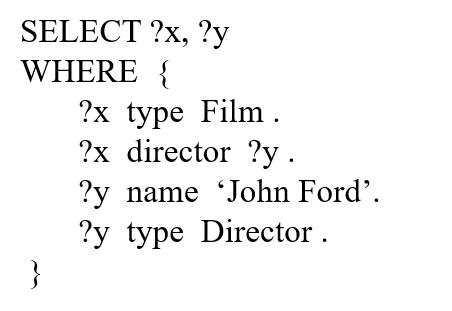
\includegraphics[width=1.6in]{query.png}
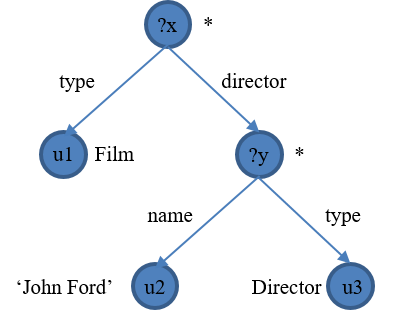
\includegraphics[width=1.4in]{query-tree.png}


\begin{center}
(a) SPARQL Query\ \ \ \ \ \ \ \ \ \ \ \ \ \ \ \ \ \ \ (b) Query Tree
\end{center}

\begin{center}
\textbf{Figure 1: User SPARQL Query}
\end{center}

In the most general case, the reason for an object missing from the result set may be various. In Example 1, the film may not be directed by \emph{John Ford}, or the film does not have the \emph{director} property in DBpedia, or even worse that the film is absent from the data set. Users may become frustrated after many times trial and error with modifying the queries. This situation motivates us to explain certain missing answers for the users in RDF data, so that they can either gain confidence about the query result or understand why the expected item is absent.

\textbf{Our Contribution} is firstly to utilize the graph pattern matching methods to answering why-not questions over RDF data. To make the algorithms be practical, we propose a unified explanation framework which allows user to pose why-not questions and seek clarifications. Besides, we propose several optimization strategies to accelerate the explaining process and reduce the computation cost. Moreover, we design and conduct series of experiments to evaluate our framework. The experimental results confirms that our approach can achieve the state-of-the-art effect by generating satisfactory answers for the why-not questions efficiently.

The rest of paper is organised as follows. Section 2 will presents the related work in solving why-not problems. The proposed explanation framework and detailed methodology will be illustrated in Section 3. Section 4 will demonstrate some optimization strategies based on the pre-defined framework. Section 5 covers the experimental study. We draw the conclusions and discuss the future work in Section 6.


\section{Related Work}

Answering why-not questions has received much attention in the database community and been extensively studied in recent years. In this section, we mainly review previous work on why-not questions with different data and query settings.

\textbf{Why-not Questions on Relational Database.} The first fundamental work on why-not questions can be found in \cite{bgf:chapman2009not} proposed by Chapman and Jagadish. Since then, various kinds of methods are designed for answering why-not questions. The existing approaches can be classified into three categories: (i) manipulation identification \cite{bgf:chapman2009not,bidoit2014query}, which aims to find the operators in the user query that are responsible for non-answers. (ii) database modification \cite{huang2008provenance,herschel2010explaining,herschel2009artemis}, which gives a way to explore the derivation of why-not tuples and modify the database such that missing answers can appear in the result set of user query after modification. (iii) query refinement \cite{tran2010conquer,he2014answering,islam2013answering}, which tries to change the primitive query and generate a new refined query with the minimum cost, thus the new query can include both original query results and user-expected answers. It is worth noting that, all these approaches focus on computing explanations on relational database. As data structures of different databases may be totally disparate, these techniques are not applicable on other databases, e.g. graph, social, XML, RDF etc.

%\textbf{Query Mechanisms.} Why-not questions are query-dependent, for this reason, different query settings are required for different queries. Islam et al. \cite{islam2013onanswering} summarize a comprehensive list of query types on why-not questions. Thus far, various queries have been investigated over relational database, such as SPJ \cite{bgf:chapman2009not,huang2008provenance}, SPJA \cite{tran2010conquer}, SPJUA \cite{herschel2010explaining}, top-k queries \cite{he2014answering}, reverse top-k queries \cite{gao2015answering} and reverse skyline queries \cite{islam2013answering}, etc. Nonetheless, all these studies aim to answer why-not questions with refined queries on relational database, and just cover a portion of the query list. On this account, these approaches would fail on processing other queries on a different database, e.g. graph queries on a graph database.

\textbf{Why-not Questions on RDF Data.} Answering queries on graph-structured data has been a research hotspot recently. As graph queries are always so strict that the query result may be small or empty, researchers are making efforts to relax the origin query to attain more related results. According to the modification style, techniques mainly fall into three categories: (i) query relaxation \cite{koudas2006relaxing,huang2008computing,elbassuoni2011query}, which generalizes the classes and properties through RDF(s) entailment to relax the constraints. (ii) query approximation \cite{grahne2006regular,huang2012approximating}, using flexible matchings to make more items being matched. (iii) combined approach \cite{poulovassilis2010combining}. However, the target of these research is obtaining much more related answers, rather than making plausible explanations. To answer why-not questions over graph data, a recent work \cite{islam2015efficient} proposed an approach of modifying the initial query into a new query which includes the missing graphs in the answer set. However, the data settings in this work has no relation with RDF. To the best of our knowledge, why-not questions over RDF data is not effectively addressed in the existing literature.

%\textbf{Graph Matching.} The purpose of Graph matching is to enumerate all the matches of a query pattern on a global graph. The query pattern may be different types, including a tree \cite{chen2005stack,chang2015optimal}, a directed acyclic graph \cite{chen2005stack}, or a general graph \cite{cheng2008fast,laiscalable}. According to the matching styles, the graph matching problem can be divided into three categories: (i) subgraph isomorphism \cite{shang2008taming,zhu2012treespan}, this kind of matching is a one-to-one mapping from nodes and edges of query pattern to nodes and edges of data graph. Apparently, it may be too restrictive to identify patterns. (ii) pattern matching \cite{chen2005stack,cheng2008fast,bruno2002holistic,cheng2013top,gou2008efficient}, which relaxes the matching condition by mapping edges of query pattern to feasible path in a graph. (iii) graph simulation \cite{fan2010graph,fan2013diversified}, which enumerates all binary relations between query nodes and matched graph nodes. It is worth mentioning that all these studies are not directly related to the why-not question, but they make contributions when studying the why-not problem on graph database with a graph query.

%The requirement of answering why-not questions are not merely appearing on relational database, but also on other types of database, such as graph, social, XML, and RDF etc. In this work, we study the why-not problem on a new situation, specifically, on a graph database (data structured as RDF triples) with graph query (in sparql format). As why-not questions are query-dependent, this work is completely different from those on relational database with sql query. Our goal is to generate appropriate explanations when users propose the why-not questions on RDF graph database.

In this work, we address the problem of answering why-not questions to sparql queries over RDF data via constructing a new query with a novel graph pattern matching approach. The constructed query can include the missing answers as well as maximize the similarity with original user query. With the method, the users can obtain quality explanations for the missing items and also, garner better understanding over the query.

\section{Explaining Why-not Questions}

\subsection{Problem Statement}

In this paper, we work with RDF graphs which is a collection of subject-property-object(SPO) triples.
Assume there are infinite sets $I$(IRIs), $B$(blank nodes) and $L$(RDF literals), then each triple $t$ formed
as $(s,p,o) \in (I \cup B) \times I \times (I \cup B \cup L)$ is either a pair of entities with a named relationship or an entity with named attribute and value.
For user queries, we mainly consider the basic select-project-join(SPJ) fragment of sparql queries
where the selection condition is a conjunction of triple patterns $P_1 \wedge \cdots \wedge P_l$.
Each $P_i$ is either a selection triple pattern ��$(S_j$ $op$ $c)$�� or a join triple pattern ��$(S_j$ $op$ $S_k)$��,
where $S_i$ is either a resource standing for either an entity or a variable, $c$ is a literal, and $op$ is a predicate.

\textbf{\underline{Why-not Questions.}} Given an input sparql query $Q$ on a RDF graph $G$, let $Q(G)$ denote the result set of $Q$ on $G$. In the most basic form, a why-not question on $Q(G)$ is represented by a non-empty collection of why-not keywords $K=\{k_1, \cdots, k_n \},n \geq 1$, where each why-not keyword $k_i$ can be mapped on $G$ with an entity $e_i$ and $e_i \notin Q(G)$. Corresponding to the why-not keywords, why-not instances is denoted as a non-empty set of instances $I=\{e_1, \cdots, e_n\}$.

Essentially, the why-not question is asking why $I$ is not a subset of $Q(G)$; i.e., why each $e_i \in I$ is not in $Q(G)$. In the most general case, a user sparql query may contain multiple variables, thus a why-not question may be posed towards different variables which might cause ambiguity. By default, the select clause of sparql query limits the returned result and why-not questions are associated with the selected variables naturally. For simplicity and without loss of generality, we assume each why-not keyword responds to a specific variable within the user sparql query. Therefore, a why-not question on $Q(G)$ is represented by $WN=\{(k_1,v_1 ), \cdots ,(k_n,v_n)\},n \geq 1$ where each why-not pair $(k_i,v_i)$ is a why-not keyword $k_i$ and its related variable $v_i$. The default circumstance can be easily processed as the responding variable $v_i$ is set to $null$. In Example 1, the why-not keyword is \emph{Dreamboy}, corresponding why-not instance mapped on the RDF Graph is \emph{http://dbpedia.org/resource/Dreamboy}, the why-not question is represented by $WN=\{("Dreamboy", ?x)\}$.

\textbf{\underline{Query Pattern.}} Given a sparql query $Q$, the main component of $Q$ is the where clause which is a conjunction of triple patterns. Assume there is a set of variables $V$ disjoint from the sets $I$, $B$ and $L$, then each triple pattern is a triple $(v_1,v_2,v_3 ) \in (I \cup V) \times (I \cup V) \times (I \cup V \cup L)$. A query pattern is a set of triple patterns where the same variable in different patterns denotes a join condition. As a triple pattern can be viewed as a directed edge, a query pattern can be represented as a tree structure. In Example 1, the query pattern of user sparql query can be depicted as a tree in Figure 1(b).

\textbf{\underline{Why-not Query.}} Given a sparql query $Q$, a why-not query $Q^*$ is a refined query which is derived from $Q$ with some modification operations. Since the modification operations may be various, we try to construct the why-not query with graph matching methods and preserve the most similar query pattern with $Q$. In essence, why-not query is a similar query pattern of $Q$ whose results contain the why-not instances.

\textbf{\underline{Explanation.}} Given a sparql query $Q$ and why-not questions $WN$,  the explanation for each why-not question is represented by $E=\{(tq_1, tw_1 ), \cdots, (tq_m, tw_m )\}, m \geq 1$, where $(tq_i, tw_i )$ is a RDF term pair, $tq_i$ is a RDF term in the user sparql query, $tw_i$ is a RDF term in the why-not query, and $tq_i \neq tw_i$. The explanation answers the why-not question by given a suggestion of modifying the RDF term $tq_i$ to a new RDF term $tw_i$. Considering example 1, we can construct a why-not query by substitute the node $u2$ in Figure 1(b) with a new node $v2$ labeled with \emph{Gilbert Perez}, and the new query can return the user-expected item \emph{Dreamboy}. Thus we can return \{``John Ford'', ``Gilbert Perez''\} as an explanation, which informs that Dreamboy was not returned because its director is Gilbert Perez, not John Ford.

Given the above statements, we formalize the problem of answering why-not questions to sparql queries on RDF databases as follows: Given an input sparql query $Q$, a RDF graph $G$, and why-not questions $WN$, the process of seeking why-not answers is to compute a reasonable explanation $E$. According to the explanation, users can either understand why her interested item is not in the result set or try to change the original query to gain the expected instances.

\subsection{Framework and Algorithms}

In this section, we propose a unified framework called $WQSQ$ (i.e., \textbf{W}hy-not \textbf{Q}uestions on \textbf{S}parql \textbf{Q}ueries) and present an overview of our approach to compute explanations for why-not questions by heuristically generating a refined why-not query. As illustrated in Figure 3, $WQSQ$ takes a sparql query, a RDF graph and why-not questions as input, and returns the refined sparql query with maximum similarity to users. Specifically, the explanation framework mainly consists of the following three steps:
(1)	Mapping why-not keyword on RDF graph.
(2)	Constructing why-not query.
(3)	Computing explanations.
Details of the framework will be discussed subsequently.

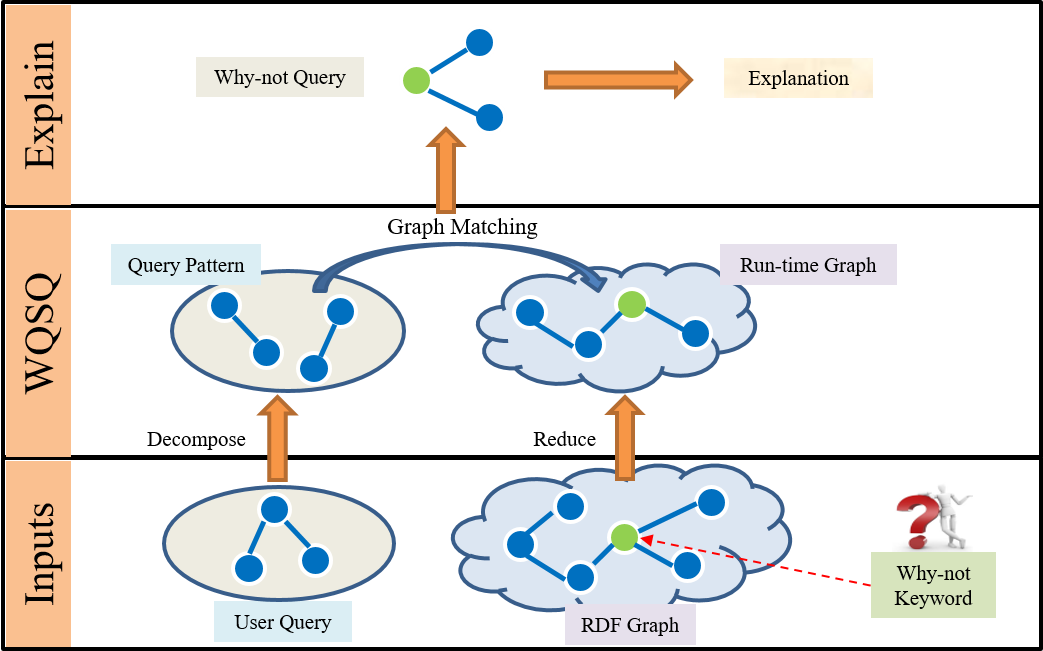
\includegraphics[width=3.36in]{framework.png}

\begin{center}
\textbf{Figure 3: Framework of WQSQ}
\end{center}

In the first step, we need to find the correct instance in the RDF graph the why-not keyword mapped. A simple way is to search the keyword on the RDF graph and return the instance whose certain attribute value is the keyword. As the search method is executed as an exact matching process, this method always return empty or irrelevant results. For another aspect, if we use a similarity-based method to obtain all relevant instances whose value is similar with the keyword, then too many results would be returned. As a compromise, we use the latter approach to get some instances with a similarity threshold $\tau$ limited. After that, the syntax information of edges in the query pattern is exploited to disambiguate the instance. Consequently, only a few instances are mapped from the why-not keyword to the RDF graph, and we can utilize the similarity score of the final constructed why-not query to further differentiate them. It is worth noted that, if no instances are mapped with the why-not keyword, then the framework finished at this step because it's meaningless to explain an nonexistent instance in the RDF graph.

In the second step, we present a graph pattern matching method to construct a why-not query, which is outlined in Algorithm 1. Before the matching procedure, we decompose the query to several graph patterns(Line 1). The advantage of the pattern decomposition is that the whole matching procedure can be divided into series of iterations, where each iteration corresponds to a subgraph pattern matching. Hence the median results generated by each iteration can be sorted with a similarity score and utilized to guide the matching direction. That is, the matching process are ensured to obtain the most similar subgraph with the query pattern in each iteration, which also makes the final matched graph have a maximum similarity score with the user query. Several techniques for graph pattern matching has been proposed, such as edge based, star based, multi-way based, twin-twig based approaches. In this paper, we adopt the edge based approach for simplicity and efficiency. The matching process starts from the why-not instance, so that we can guarantee that the final constructed why-not query can return the user expected item. In the first iteration, we execute the match between all edges linked with why-not instance and all query patterns. Each matching pair between a random edge and a query pattern is assigned with a similarity score by the score function. Then we obtain the match pair with highest similarity score and expand the node by adding the linked edges into the candidate edges collection. Following during each matching process(lines 5-7), we compute the similarity score between candidate edges and remainder query patterns(line 6). Then we find the most similar edge to join into the matching subgraph generated in the former iteration(line 7). At last, a tree structure which is similar to the user query rooted at the why-not instance is constructed. With the corresponding nodes being replaced by different variables(line 9), a why-not query is generated.

\begin{algorithm}         %�㷨�Ŀ�ʼ
\caption{ Construct a why-not query.} %�㷨�ı���

\KwIn{Run-time Graph, $G_R$; User Sparql Query, $Q$; Why-not Instances of a certain keyword, $WI=\{wi_1,wi_2,\cdots,wi_m\}$}
\KwOut{Why-not Query, $Q_w$}

Decompose $Q$ into edges pattern $P=\{p_0, p_1, \cdots, p_l\}$;
Initial similar graph collection $G_s \leftarrow \emptyset $;\\
\For {each why-not instance $wi_j \in WI$}
{
     $G_j=(N_j, M_j);$  $N_j=\{wi_j\}$, $M_j=\emptyset;$  $score=0;$

     \For {each pattern $p_i \in P $}
     {
          \For {each edge $e$ in linked edges of unmatched node $v$ in $N_j$}
          {
               compute similarity score between $e$ and $p_i$;
          }
     }
     $score += maximum\{sim(e, p_i)\};$
     $M_j.join(e);$  $N_j.add(e.neighbor(v));$
     $G_s.push(G_j);$
}
$sort(G_s);$  $Q_w=G_s.top1;$\\
replace the why-not instance in $Q_w$ with a variable $?x$;\\
return $Q_w$;                %�㷨�ķ���ֵ

\end{algorithm}

%Lemma 1: The space complexity and time complexity of Algorithm 1 are O() and O() respectively.

%Proof Sketch:

After the why-not query is generated, we can return this refined query to the users as an answer to the why-not questions. However, the explanation is a little vague because of the coarsness. Thus we refined our work to compute a more fine-grained explanation. The key idea is that we make a comparison of constructed why-not query and user query. It is obvious that the two queries are not equal. As each triple in the why-not query is matched with a triple pattern in the query, we traverse the query tree, and compare the matched edge in why-not query with the triple pattern. For the labels of nodes and edges, each different place is picked out as a term pair to consist of the final explanation.

%To exemplify above, considering the example 1, we map the keyword \emph{Dreamboy} on the RDF graph firstly and get the collection of why-not instances, 

\subsection{Score Function}

In Algorithm 1, for each why-not instance, we construct a why-not query that can generate results containing the instance. Also we need the constructed query to be the most similar one to the user query. To ensure that we can obtain the best match in each iteration, a score function that measures the similarity between currently constructed subgraph and query pattern is defined as follows. For each iteration, the score of currently matched sub-graph $Gs_i$ is computed by the following formula (1-1),
$$ score(Gs_i) = score(Gs_{i-1}) + max{sim(t, p_i  )}, (1-1)$$
$$ score(Gs_0) = 0$$
where $p_i$ is the current selected triple pattern in the query, t is a candidate edge to be matched. And the similarity score between a candidate edge and a triple pattern, which are both triples, can be computed by the sum of similarity score for each term pair. Formally,
$$ sim(t, p) = sim(t_s, p_s ) + sim(t_p, p_p ) + sim(t_o, p_o ) ,$$
is the similarity degree between an edge $t$ and sub pattern $p_i$ . The similarity of each term pair can be measured by a random distance metric.

\newtheorem{thm}{Theorem}[section]
\begin{thm}
Given the score function defined by equation (1-1), the problem of constructing why-not query can be reduced to a dynamic programming problem.
\end{thm}

\textbf{Proof Sketch:} In algorithm theory, a dynamic programming problem must have two key attributes, which are optimal substructure and overlapping sub-problems, respectively. To prove this theorem, we verify whether the why-not query constructing problem satisfies the conditions from the following two aspects:
(1) Optimal Substructure. Suppose the size of decomposed patterns is $t$, and after $i$ times matching, the constructed subgraph is $Gs_i$ with currently maximum score, $score(M_i)$. In next iteration, we explore the solution space to find an edge that is the most similar with query pattern $p_i$, which makes the second addend of formula (1-1) maximized, then $score(M_{i+1})$ is maximized, the matched edge is selected and joined to $Gs_i$ to generate $Gs_{i+1}$. Hence, the solution to a given optimization problem can be obtained by the combination of optimal solutions to its sub-problems.
(2) Overlapping Sub-problems. The process of constructing the why-not query can be decomposed as a series of subroutines, we find a matched edge of a given query pattern and join into currently constructed subgraph. Suppose the final why-not graph is $Gs = e_1 \bowtie e_2 \bowtie \cdots \bowtie e_n$, then for the $i$th iteration, its sub-problems corresponding to constructing a subgraph with matched edges contain a random composition of joint $(i-1)$ edges. That is, for different iterations, the sub-problems may be overlapping.
Based on (1) and (2), the problem of constructing a why-not query satisfies the quality of optimal substructure and overlapping sub-problems, thus can be reduced to a dynamic programming problem, Theorem 3.1 holds.

From theorem 3.1, it is easy to deduce that with the well-defined score function, we can always find the most optimal solution in global. This guarantees that our algorithm can work in a correct and reasonable way.


\section{Optimization Strategies}

\subsection{Run-time Graph Construction}

Instead of loading the whole RDF graph $G$ into the main memory, we propose a method to load in a subgraph of $G$ without loss of useful information, which is called the run-time graph $G_R$ regarding user query $Q$. Considering the why-not question answering procedure, the useful information mainly covers the following two types of instance :

\begin{itemize}
\item Type-1 instance: mapped on the RDF graph by the why not keyword in the why-not question ,
\item Type-2 instance: covered by classes in the user query.
\end{itemize}

Besides, the relation between the two kinds of instance is also useful as we want to construct a query whose result covers the original instance and why-not instance as much as possible. Therefore, we extract the two kinds of instances at first, then add the linked path between type-1 instance and type-2 instance as auxiliary information. In a further step, for each type-2 instance, we only consider the linked edges labeled the same as the predicates in query pattern. Thus we use the edge information to remove useless relations and attributes of the type-2 instances. The detailed process is presented in Algorithm 2.


\begin{algorithm}         %�㷨�Ŀ�ʼ
\caption{ Construct a run-time graph.} %�㷨�ı���

\KwIn{Global RDF Graph, $G$; User Sparql Query, $Q$; Why-not keywords, $K=\{k_1,k_2,\cdots,k_n\}$}
\KwOut{Run-time Graph, $G_R$}

$QI \leftarrow \emptyset;$  $WI \leftarrow \emptyset;$  $G_R \leftarrow \emptyset;$\\
\For {each variable $v_i$ of $Q$}
{
     query instances $QI = \rho_G(v_i)$;
}
construct query instances graph $G_QI$ with $QI$;\\
\For {each keyword $k_i \in K $}
{
     $G_{R_i} = (N_i, M_i)$; $WI_{k_i} = \rho_G(k_i)$;
     disambiguate why-not instances with edges in $Q$;\\
     \For {each instance $t \in QI$}
     {
         $N_i.add(t);$  $M_i.add$(linked edges of t);
         compute joint path $p$ between $t$ and remain instances;
         $N_i.add(p.nodes);$  $M_i.add(p.edges);$
         add nodes and edges of $G_QI$ into $G_{R_i}$;
     }
     $G_R.push(G_{R_i})$;
}
return $G_R$;                %�㷨�ķ���ֵ

\end{algorithm}

%Lemma 3: The space complexity and time complexity of Algorithm 3 are O() and O() respectively.

%Proof Sketch:


\subsection{Order-aware Graph Pattern Matching}
\textbf{Definition:} (Operator $\prec$) For any two decomposed edge patterns $p_i$  and $p_j$ in $Q$, $p_i \prec p_j$ if and only if one of the three conditions holds:
\begin{itemize}
\item $d(p_i) < d(p_j)$ ;
\item $d(p_i) = d(p_j)$ , $|\sigma_G (p_i)| < |\sigma_G (p_j)|$ ;
\item $d(p_i) = d(p_j)$ , $|\sigma_G (p_i )| = |\sigma_G (p_j)|$ , $id(p_i ) < id(p_j )$ .
\end{itemize}

where $d(p_i)$ is the depth of $p_i$ in the query tree, $|\sigma_G(p_i)|$ is the frequency of occurrences of triple pattern $p_i$ in the RDF graph, and $id(p_i)$ is the unique identifier of pattern $p_i$ assigned with an integer. We utilize the hierarchy and term frequency of query pattern to define a partial ordering relation. With the defined rules, the pattern matching process can be guided in an efficient way as the searching space is reduced contrast to the full matching without order.

Intuitively, as the query can be regarded as a tree, it is helpful to match the pattern with shallow and exact information earlier. For the first aspect, the why-not instance is more likely to be the root node or in a top layer, therefore, choosing the edge pattern with lower depth in prior is better than the edge pattern with deeper depth. This can be depicted by the first condition. For another part, if two patterns have the same depth, then the pattern with lower frequency of occurrence is better because of the lower space to be selected. This can be described by the second condition. At last, if the depth and frequency are accidently the same, then it��s not important to choose which pattern to be matched, thus we just use the pattern id to differentiate the patterns, which is reflected by the third condition. 
%By the above analysis, it is apparently the order-aware pattern matching is better than no orders as the former reduce the unrelated matches in each iteration as much as possible.
%\end{Proof}

\section{Experiments and Evaluation}

In this section, we conduct the experimental study of our algorithms. First we give the instruction to set up our experiment environment, which contains the preparation of dataset, user queries and corresponding why-not questions. Then we give the evaluation of the experiments.

\subsection{Sets Up}

\textbf{Dataset.} To evaluate and validate our proposed explanation framework, a dataset is installed by selecting the main branches of data from DBpedia. Without loss of data volume, information coverage and diversity, we abandon the data files which describes only few attributes of instances(e.g. files concerning homepage and category), and combine the schema-layer knowledge and instance-layer information together to generate a jena TDB as our backend RDF graph database. The constructed database contains 82 218 699 triples, about 10.4 GB size and accounts for nearly 17.3\% of the whole DBpedia data.

\textbf{Query Set.} From this dataset, about 20 queries are constructed with each query attached with 1-3 different why-not questions. To reduce the manual factor, the queries are extracted from QALD-5\footnote{http://greententacle.techfak.uni-bielefeld.de/~cunger/qald/index.php?x=home\&q=5} sparql benchmark with SPJ format. To keep the queries distributed with uniformity, we make some change to the selected queries so that the number of queries with different complexity are close. The statistical number of queries are presented in Table 1. Subsequently, we run these sparql queries on the Virtuoso SPARQL Query Editor\footnote{http://dbpedia.org/sparql}, according to the returned results, we design the why-not questions based on the personal prior knowledge of missing answers. Consequently, we obtain  why-not questions in total.\\

\begin{tabular*}{1.53in}{|c|c|c|}
  \hline
  % after \\: \hline or \cline{col1-col2} \cline{col3-col4} ...
  \scriptsize{\#triples} & \scriptsize{\#queries} & \scriptsize{\#questions} \\
  \hline
  1 & 5 & 12 \\
  2 & 6 & 12 \\
  3 & 4 & 10 \\
  4 & 4 & 8 \\
  5 & 3 & 6 \\
  \hline
  Total & 22 & 48 \\
  \hline
\end{tabular*}
\begin{tabular*}{1.64in}{|c|c|c|}
  \hline
  % after \\: \hline or \cline{col1-col2} \cline{col3-col4} ...
  \scriptsize{\#variables} & \scriptsize{\#queries} & \scriptsize{\#questions} \\
  \hline
  1 & 10 & 24 \\
  2 & 8 & 17 \\
  3 & 4 & 7 \\
  \hline
  Total & 22 & 48 \\
  \hline
\end{tabular*}\\

\textbf{Table 1: Number of queries and why-not questions with different complexity}\\

\subsection{Evaluation}

\textbf{Eval-I: Pre-Computation Cost of Constructing Run-time Graph.} The size and computation time of constructed run-time graph for each query are shown in Figure 4. Since the why-not keyword is mapped with just serval instances, the size of run-time graph is to a large extent dependent on the size of result set of user query. In the most case, the constructed run-time graph only consists of no more than 600 nodes and 1000 edges, which is rather smaller than the whole graph with millions of nodes and edges. The algorithms have to run on the whole dataset and always costs expensively. However, constructing a run-time graph only needs about 4-7 seconds in the usual case. With the help of run-time graph, it is always possible to compute explanations for why-not questions within a second in the majority case. Note that the pre-computation is conducted off-line.

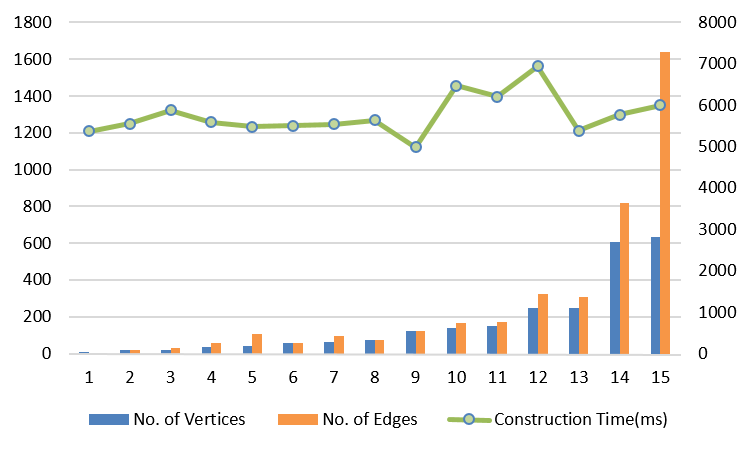
\includegraphics[width=3.1in]{run-time.png}
\begin{center}
\textbf{Figure 4: Size and construction time of run-time graph}
\end{center}

\textbf{Eval-II: Efficiency of Algorithms over DBpedia.} We use the DBpedia data to created a jena TDB as our RDF graph database, and run two algorithms(i.e., Alg1 and Alg2) with all the 48 why-not test case. We evaluate the efficiency of algorithms over all the queries. Figure 5 shows the total running time of two algorithms on different queries corresponding to the queries in Figure 4. As demonstrated, both Alg1 and Alg2 can obtain the explanations for each why-not questions within 2 seconds in most circumstance. With the order-based optimization strategy, Alg2 appears to accelerate the explaining process while shrinking about half the time of Alg1. This also proves that our order-based graph matching method can reduce the solution space theorem 4.1 informed.

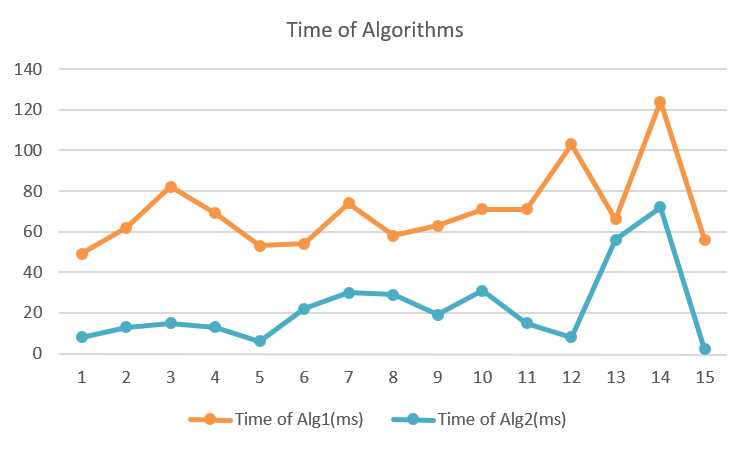
\includegraphics[width=3.1in]{alg-cost.png}
\begin{center}
\textbf{Figure 5: Time of computing explanations with different algorithms}
\end{center}

\textbf{Eval-III: The rationality of explanations.} Traditional approaches concerning rationality of why-not explanations mainly consider two aspects. One is the user satisfaction, the other is the ratio of common items in result sets of both original query and refined query. The former approach mainly takes the users' subjective judgement into account while the latter method gives an objective evaluation standard. However, the second approach is not suitable in our circumstance because sparql queries correspond to exact graph matching process and the result set of refined sparql queries always contain few items in the original result set, which would makes the recall in a low level. Hence, we only evaluate the user satisfaction for why-not queries in this study.

To guarantee that the feedback really reflects the user satisfaction, we set up the control group and test group respectively. Each group consists of 8 members who are familiar with sparql and RDF concepts. The members in control group are noticed that they are conduct a research concerning why-not problems while the members in test group are informed nothing. All the members do not know where the explanation comes from. The questionnaire is designed with 20 queries with each one given the query, why-not question and explanation. The options are made in 5 levels range from dissatisfaction to satisfaction. All the members are asked to choose an option and write down a specific percent about to what extent they feel satisfied about the explanation. Figure 6 represents the user satisfaction of queries correspond to the queries in Figure 4. It is concluded that the explanation computed by our algorithm can satisfied most of the users with an average of satisfaction degree about 81.6\%.

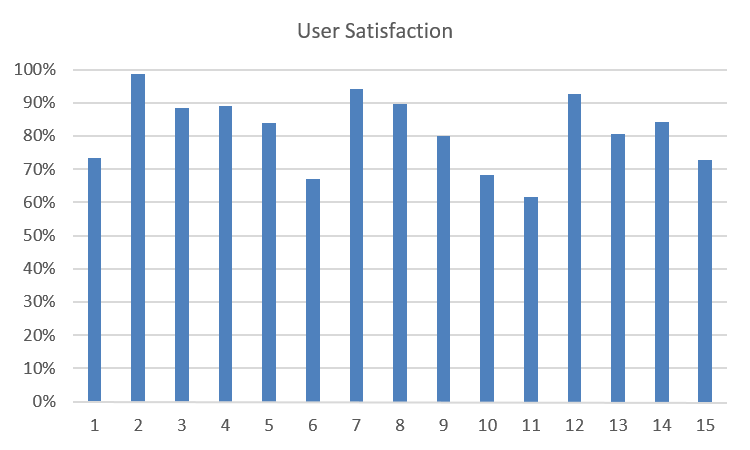
\includegraphics[width=3.1in]{rationality.png}
\begin{center}
\textbf{Figure 6: User satisfaction of explanations}
\end{center}

\textbf{Eval-IV: The Influence of Query Complexity.} We evaluate whether the query complexity affects the performance of algorithms or not. For a sparql query in SPJ format, query complexity is mainly embodied in the number of triples and variables. Figure 7 illustrates the time costs of Alg1 and Alg2 of queries with different number of triples and variables respectively. In figure 7(a), the time costs increase monotonically with the increment of triples number. It is worth noted that our algorithms run several iterations for each query where the number of times is equal to the size of query patterns. Therefore, while the number of triples goes up, the iteration time goes up, and then the time costs of algorithms increase followed. In figure 7(b), the time costs also increase while the variables of queries going up. It is showed that time costs of algorithms is influenced by the query complexity to some extent.

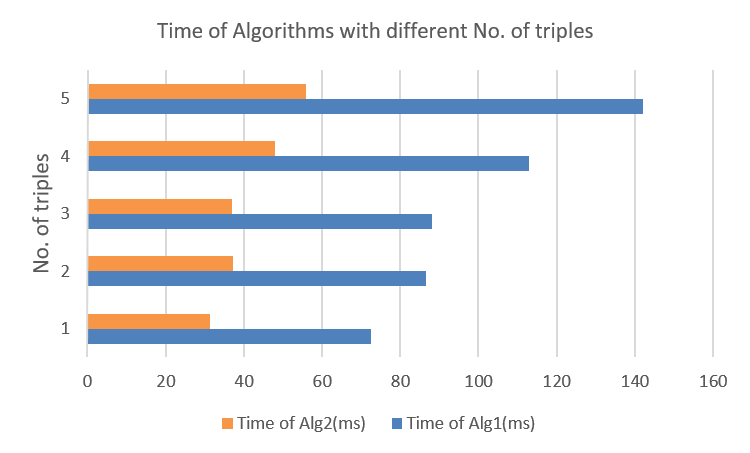
\includegraphics[width=1.6in]{Qtriples.png}
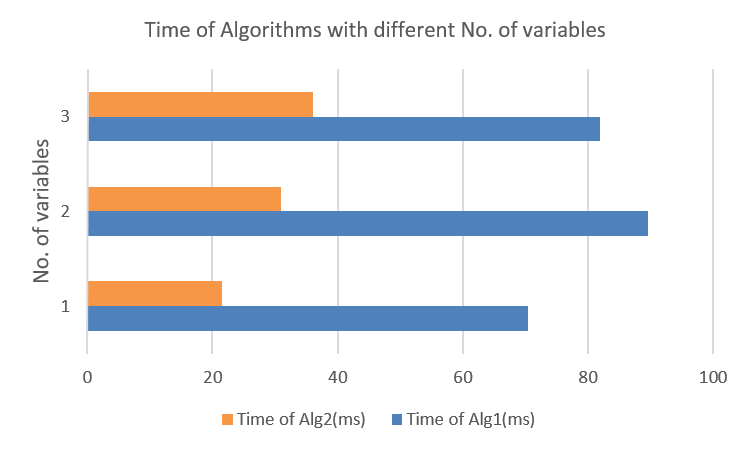
\includegraphics[width=1.6in]{Qvariables.png}
\begin{center}
\textbf{Figure 7: Time cost of different query complexity}
\end{center}

\section{Conclusion and Future Works} In this paper, we proposed an explanation framework for why-not questions on sparql queries over RDF graph databases. Our approach adequately utilize the graph structure of both database and query and adopt a graph matching method to construct a refined why-not query. To improve the performance of algorithms, we complete the framework with two optimization strategies. The experiment results demonstrate that our algorithms can answer the why-not query efficiently and satisfying the users in a high level.

Promising directions for future research include the more complicated format of queries, since our framework are limited with SPJ queries only. For a further step, it is necessary to enrich the user query by considering the union, aggregation operations. Another interesting topic is how the query pattern decomposing strategies influence the refined query. Since the edge decomposition may be a little simple, the syntax information of query might be ignored without sufficient consideration.

%% The file named.bst is a bibliography style file for BibTeX 0.99c
\bibliographystyle{named}
\bibliography{ijcai16}

\end{document}

